\section{Theorie}
\label{sec:Theorie}

\begin{figure}
  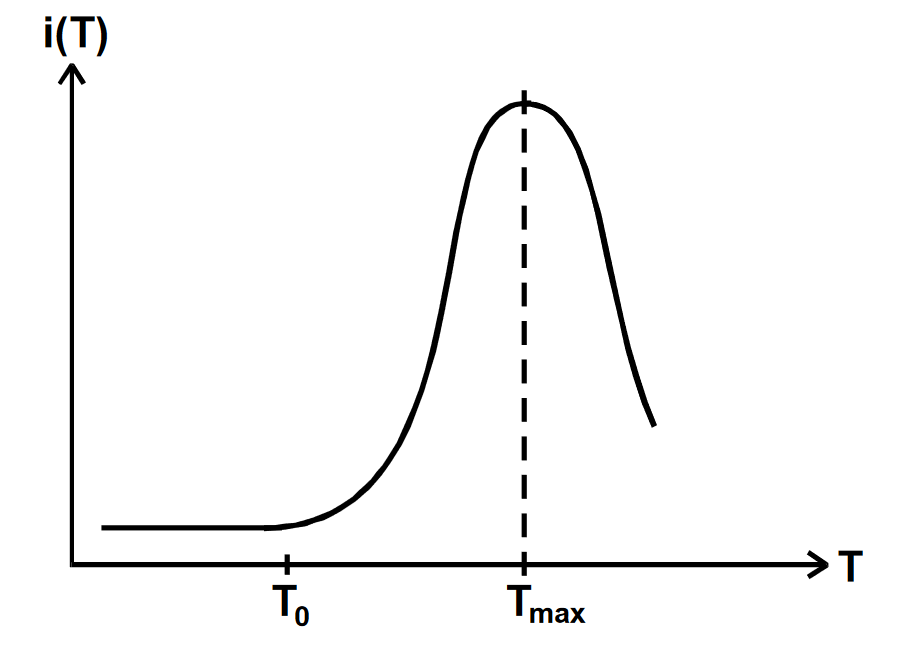
\includegraphics{./logos/Strom_theorie.PNG}
  \caption{Qualitativer erwarteter Verlauf des Dipolstromes $i(T)$.\cite{Anleitung}}
  \label{fig:strom-theo}
\end{figure}

\begin{figure}
  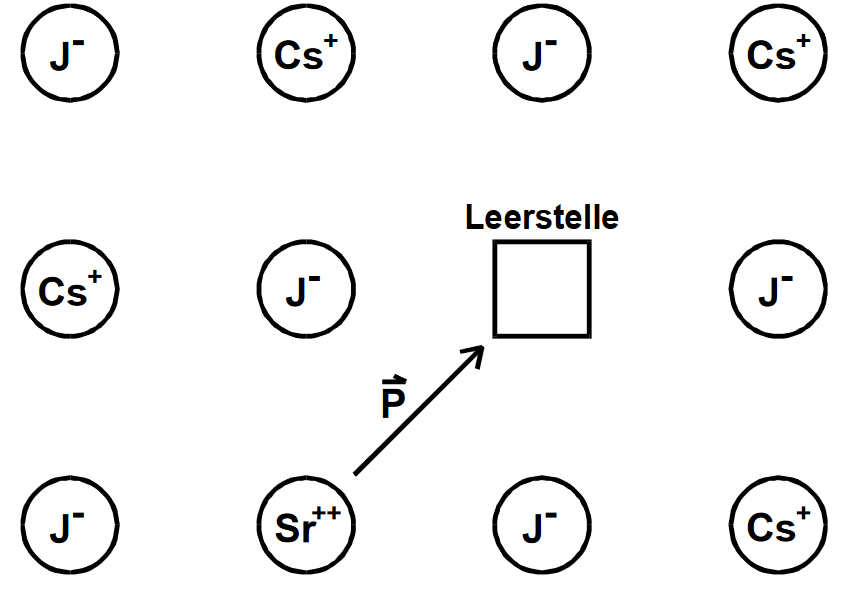
\includegraphics{./logos/Fehlstelle.PNG}
  \caption{Schematische Darstellung der Entstehung von Dipolmomenten in Kristallgittern.\cite{Anleitung}}
  \label{fig:fehlstelle}
\end{figure}
\begin{equation}
  \tau (T) = \tau_0 \exp{\left(\frac{W}{kT}\right)}
  \label{eqn:relaxation}
\end{equation}
\begin{equation}
    y(T) = \frac{pE}{3kT}
\end{equation}
\begin{equation}
  b := \frac{\symup{d}T}{\symup{d}t} = \text{const}
  \label{eqn:heizrate}
\end{equation}
\begin{equation}
  j(T) = y(T_p) \cdot p \cdot\frac{\symup{d}T}{\symup{d}t}
  \label{eqn:dichteansatz}
\end{equation}
\begin{equation}
  \frac{\symup{d}T}{\symup{d}t} = - \frac{N}{\tau(T)}
  \label{eqn:dgl}
\end{equation}
\begin{equation}
  j(T) \approx \frac{p^2 E N_p}{3kT_p\tau_0}\exp{\left(\frac{-W}{kT}\right)}
  \label{eqn:dichtefertig}
\end{equation}
\begin{equation}
  \tau(T) = \frac{\int_{T}^{\infty}i(T')\symup{d}T'}{bi(T)}
  \label{eqn:tau2}
\end{equation}
